% Chapter 1

\chapter{Implementation and Data} % Main chapter title

\label{Chapter4} % For referencing the chapter elsewhere, use \ref{Chapter1} 

\lhead{Chapter 4. \emph{Implementation and Data}} % This is for the header on each page - perhaps a shortened title

%----------------------------------------------------------------------------------------

\section{Extensions}

Our objectives are therefore the enhance some parts of the cascade. It does not, on the other hand, make sense to attempt to improve all . After all, we may assume a HEP \emph{date} is no different from dates printed in other scientific papers. The same goes for names, and with little exception\footnote{It is in fact true that collaborations feature in isolated references in HEP papers (see Section \ref{sec:futurework}).}, reference lists and their contents.

\section{Data Acquisition}

Acquiring training data for learning metadata extraction is a stupendously time-consuming task. Indeed, 

``The \emph{note} field is the one most confused with others, and upon inspection is actually labeled inconsistently in the training data''. \cite{Peng04accurateinformation}.

\section{Feature Engineering}

Baseline features should be stated 

\[
  \text{lev}_{a, b}(i, j) = 
  \begin{cases} 
  	\text{max}(i, j) &\quad\text{if min(i, j) = 0} \\
	\text{min}
		\begin{cases}
			\text{lev}_{a, b}(i - 1, j) + 1 \\
			\text{lev}_{a, b}(i, j - 1) + 1 \\
			\text{lev}_{a, b}(i - 1, j - 1) + 1_{a_i \neq b_j} \\
		\end{cases} &\quad\text{otherwise} \\
  \end{cases}
\]

Radar plots here

\begin{figure}
\centering
\begin{tabular}{cccc}
\subfloat[A]{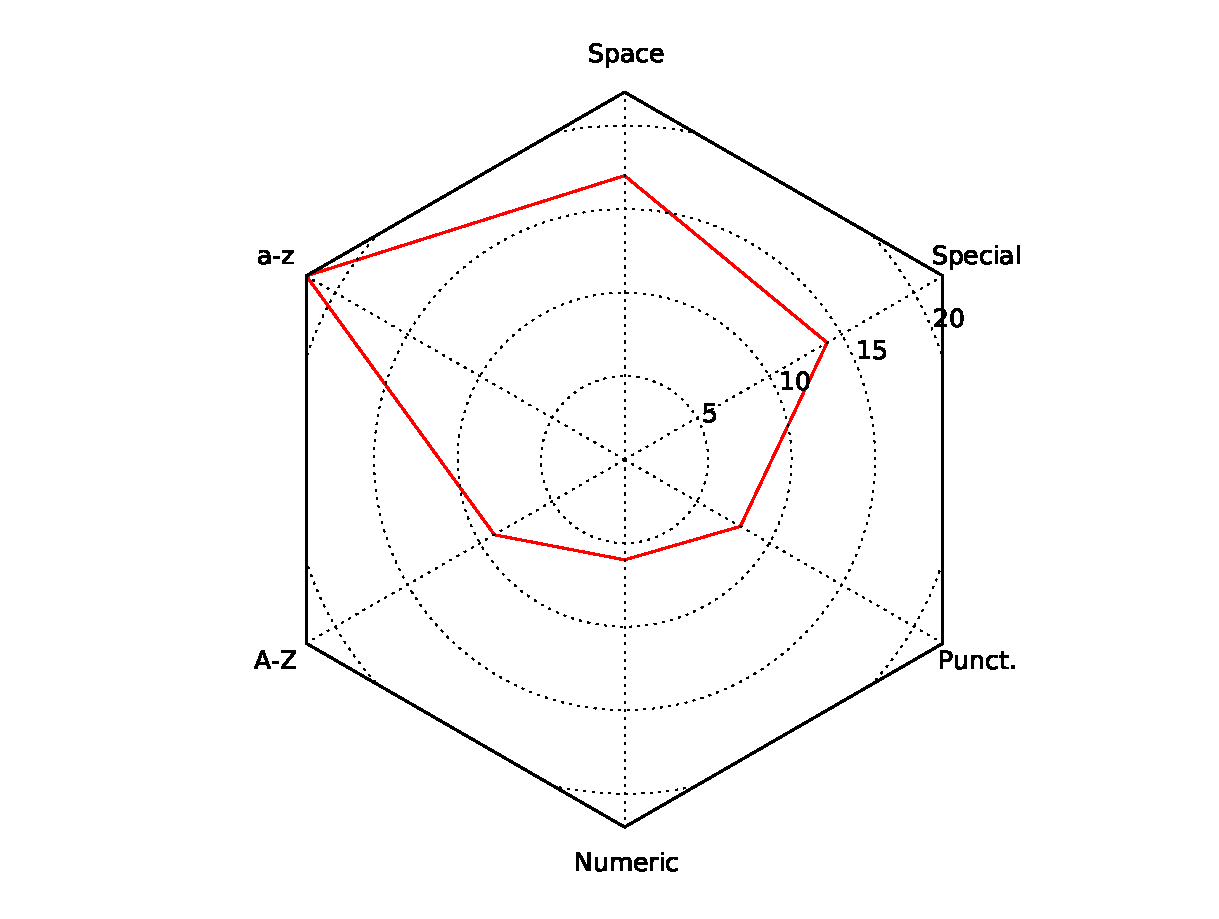
\includegraphics[width=0.5\textwidth]{Figures/body_formula.pdf}} & 
\subfloat[B]{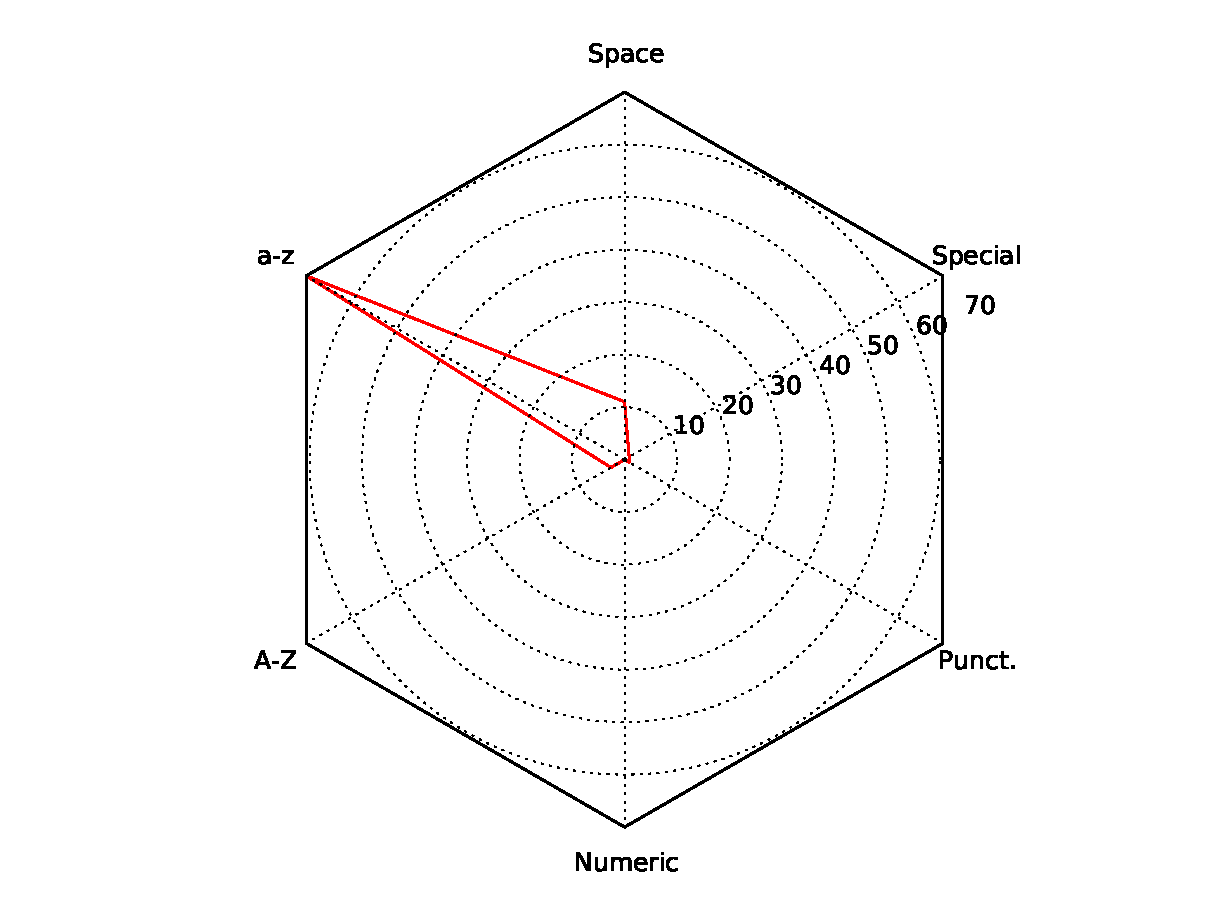
\includegraphics[width=0.5\textwidth]{Figures/body_normal.pdf}}\\
\subfloat[C]{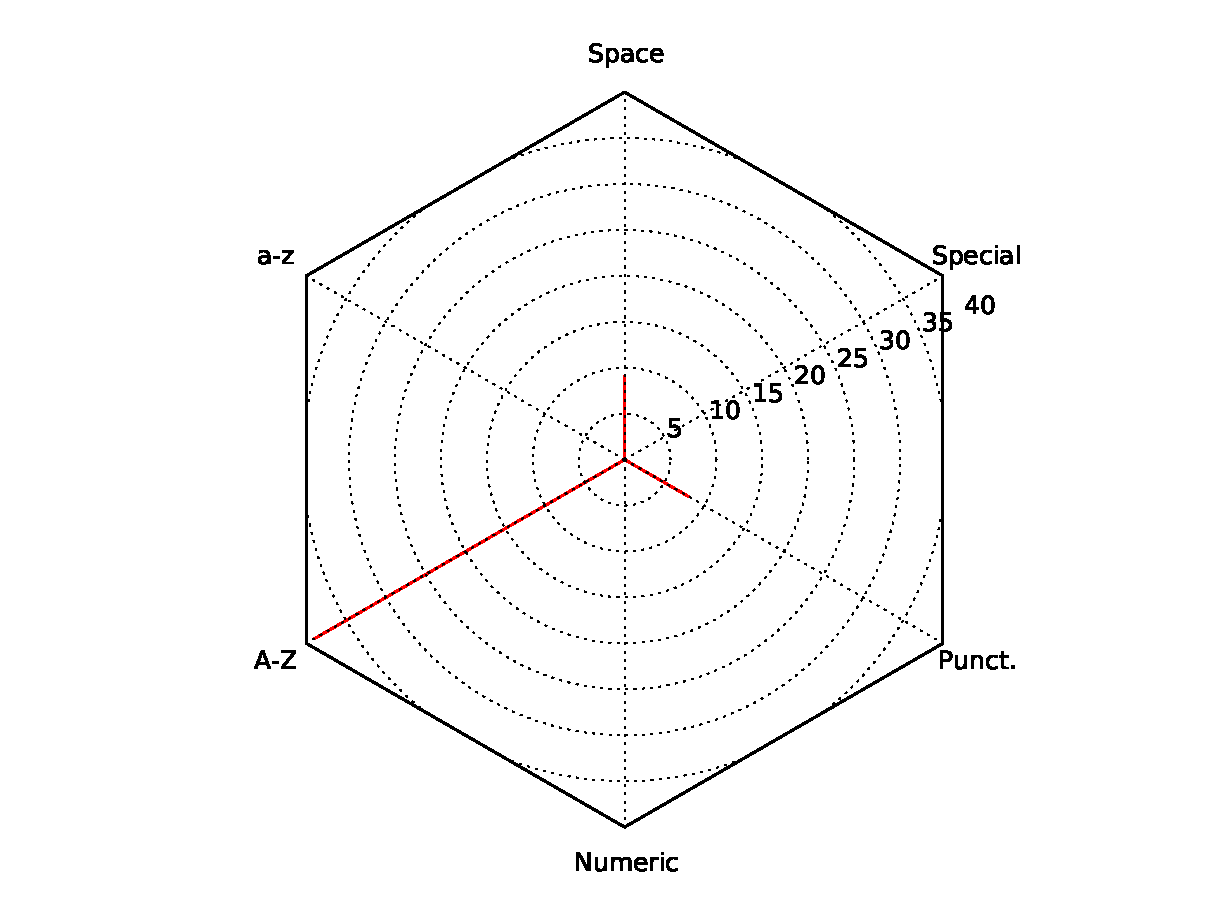
\includegraphics[width=0.5\textwidth]{Figures/headnote.pdf}}&
\subfloat[D]{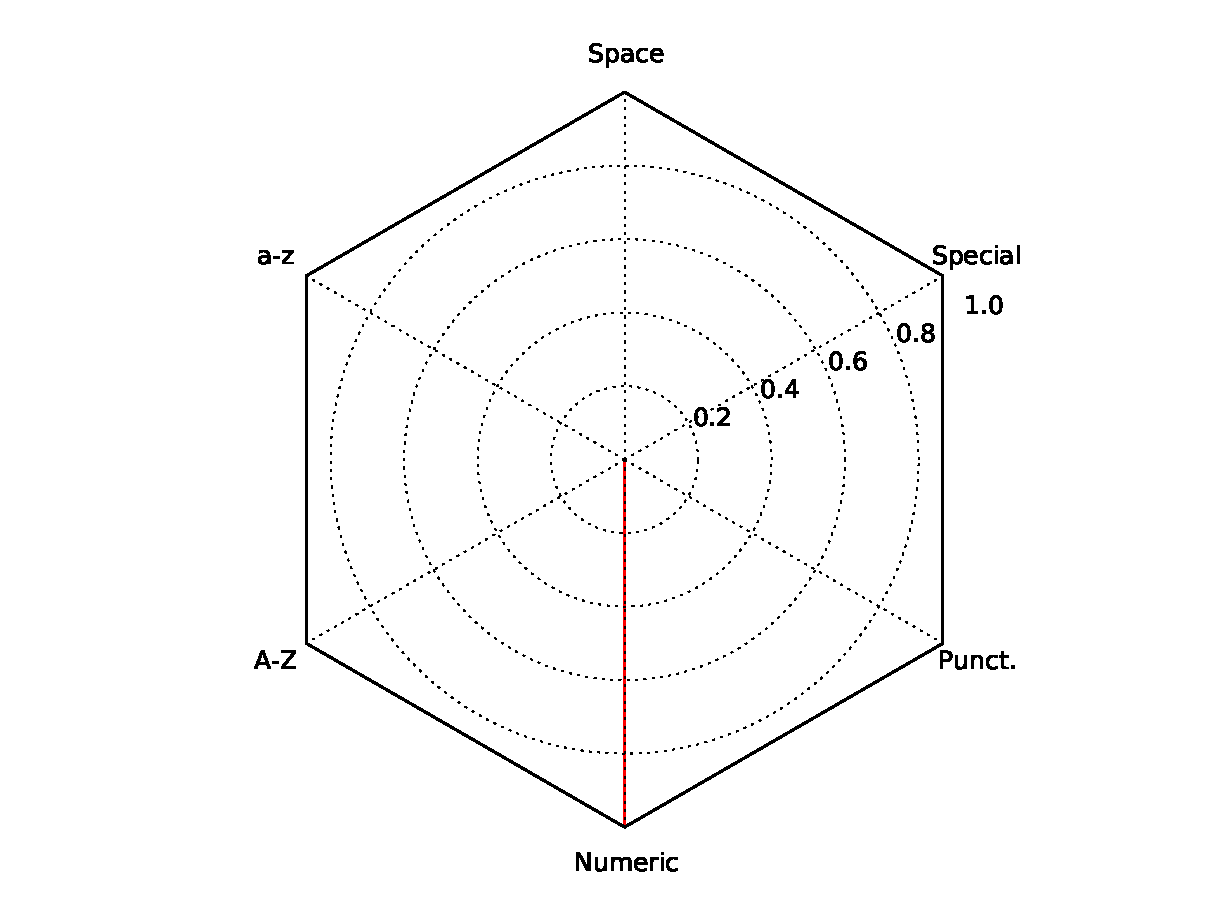
\includegraphics[width=0.5\textwidth]{Figures/page.pdf}} \\
\subfloat[E]{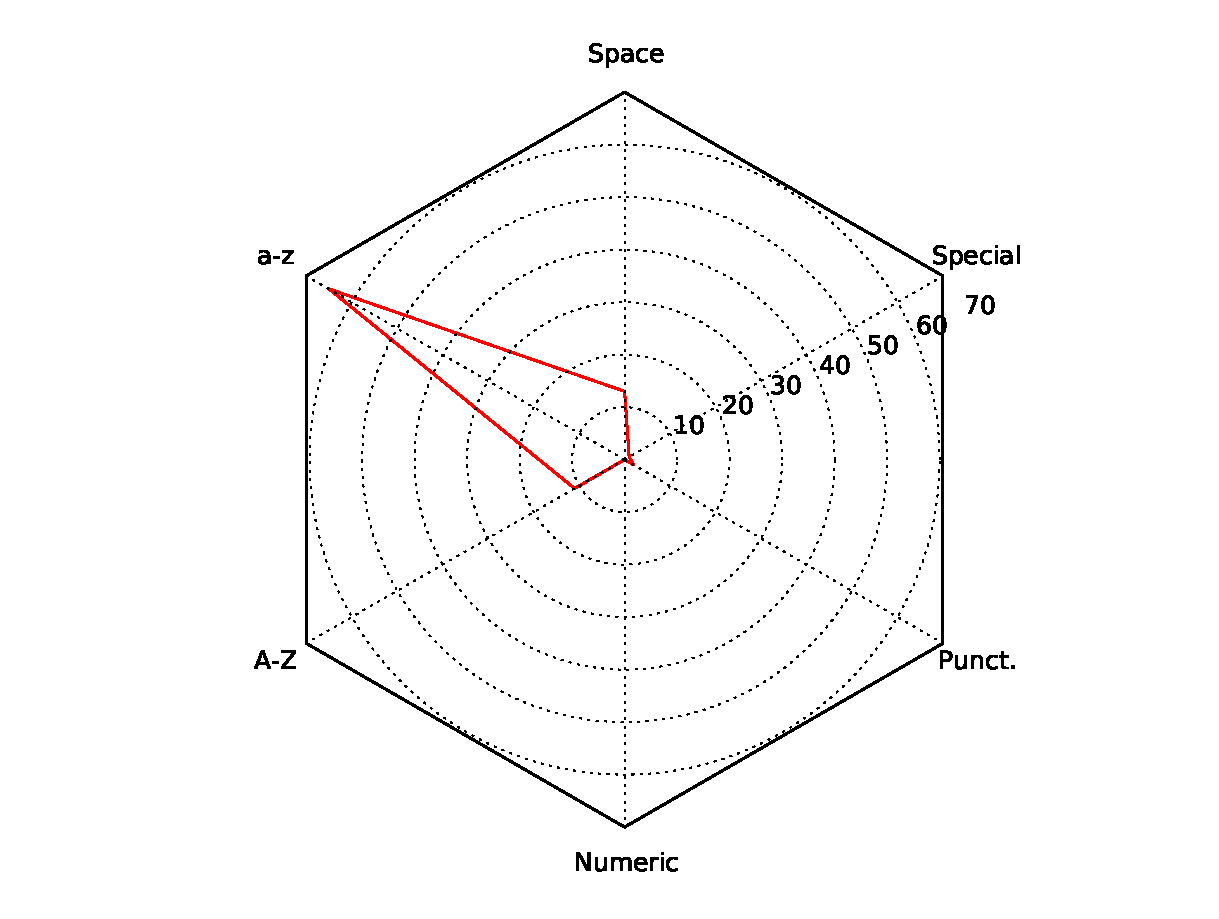
\includegraphics[width=0.5\textwidth]{Figures/affiliations_list.pdf}} & 
\subfloat[F]{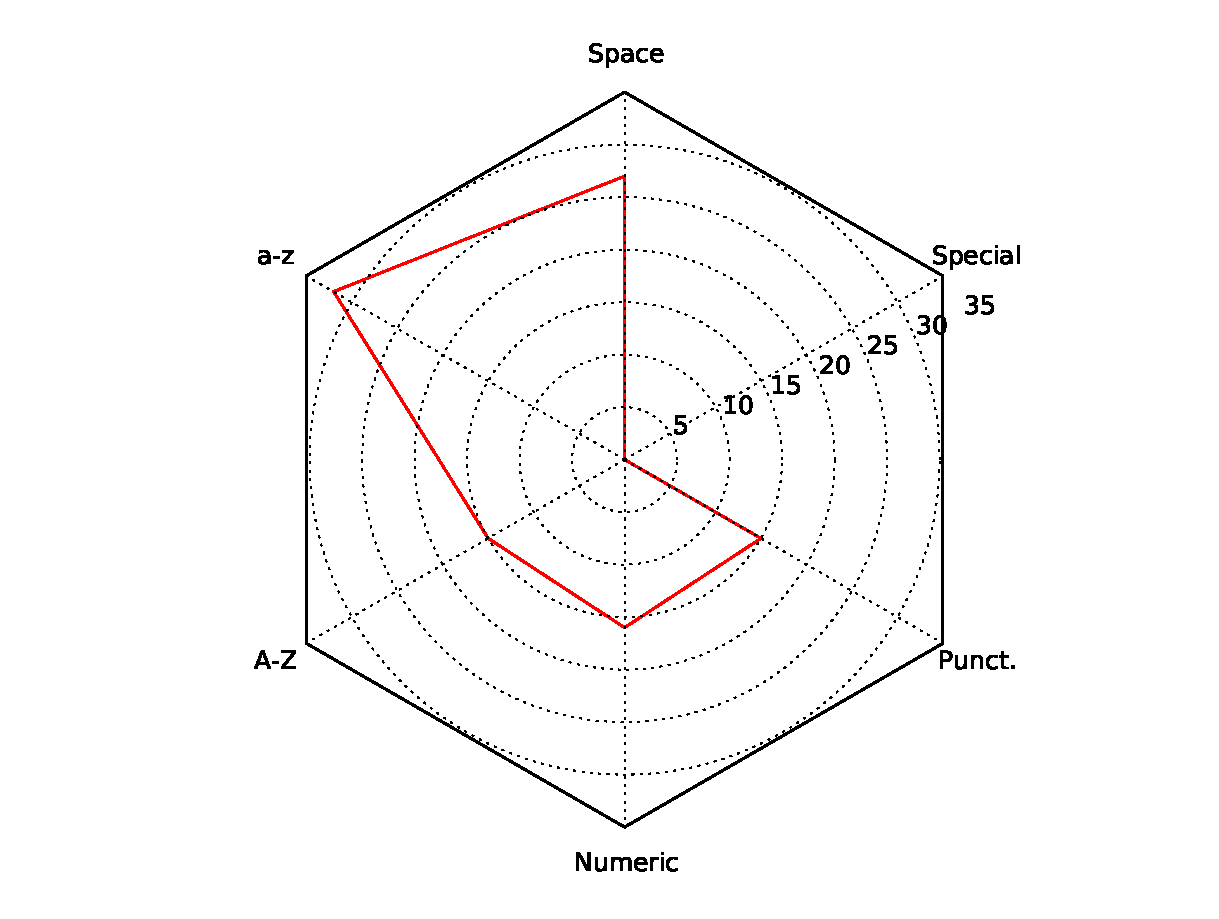
\includegraphics[width=0.5\textwidth]{Figures/author_list.pdf}} \\ 
\end{tabular}
\caption{Many figures}
\end{figure}
